\documentclass[review]{elsarticle}
\usepackage{lipsum}
\makeatletter
\def\ps@pprintTitle{%
 \let\@oddhead\@empty
 \let\@evenhead\@empty
 \def\@oddfoot{}%
 \let\@evenfoot\@oddfoot}
\makeatother
\usepackage{lineno,hyperref}
\modulolinenumbers[5]

\journal{Journal of \LaTeX\ Templates}

%%%%%%%%%%%%%%%%%%%%%%%
%% Elsevier bibliography styles
%%%%%%%%%%%%%%%%%%%%%%%
%% To change the style, put a % in front of the second line of the current style and
%% remove the % from the second line of the style you would like to use.
%%%%%%%%%%%%%%%%%%%%%%%

%% Numbered
%\bibliographystyle{model1-num-names}

%% Numbered without titles
%\bibliographystyle{model1a-num-names}

%% Harvard
%\bibliographystyle{model2-names.bst}\biboptions{authoryear}

%% Vancouver numbered
%\usepackage{numcompress}\bibliographystyle{model3-num-names}

%% Vancouver name/year
%\usepackage{numcompress}\bibliographystyle{model4-names}\biboptions{authoryear}

%% APA style
%\bibliographystyle{model5-names}\biboptions{authoryear}

%% AMA style
%\usepackage{numcompress}\bibliographystyle{model6-num-names}

%% `Elsevier LaTeX' style
\bibliographystyle{elsarticle-num-names}
\usepackage{pgfplots}
%\usepackage{natbib}
%\bibliographystyle{plainnat}
%%%%%%%%%%%%%%%%%%%%%%%

\begin{document}

\begin{frontmatter}

\title{Evaluating Performance of Clone Detection Tools in Detecting Cloned Co-change Candidates}
%\tnotetext[mytitlenote]{Put some text for title note}

%% Group authors per affiliation:
\author{Md Nadim, Manishankar Mondal, Chanchal K. Roy}
\ead{\{mdn769, mshankar.mondal, chanchal.roy\}@usask.ca}
\address{Department of Computer Science, University of Saskatchewan, Saskatoon, Canada}

\begin{abstract}
Code reuse by copying and pasting from one place to another place in a code-base is a very common scenario in software development which is also one of the most typical reasons for introducing code clones. There is a huge availability of tools to detect such cloned fragments and a lot of studies have already been done for efficient clone detection. There are also several studies for evaluating those tools considering their clone detection effectiveness. Unfortunately, we find no study which compares different clone detection tools in the perspective of detecting cloned co-change candidates during software evolution. Detecting cloned co-change candidates is essential for clone tracking. In this study, we wanted to explore this dimension of code clone research. We used 12 different configurations of nine promising clone detection tools to identify cloned co-change candidates from eight C and Java-based subject systems and evaluated the performance of those clone detection tools in detecting the cloned co-change fragments. Our findings show that a good clone detector may not perform well in detecting cloned co-change candidates. The amount of unique lines covered by clone fragments, the number of detected clone fragments, source file processing mechanism, types of detected clones plays an important role in detecting cloned co-change candidates. 
%The findings of this study can enrich a new dimension of code clone research in software engineering. 
%To select those clone detection tools and subject systems, we considered related works and popularity index of programming languages. 
\end{abstract}

\begin{keyword}
Clone Detection, Cloned Co-change Candidates, Commit operation, Software Maintenance.
\end{keyword}

\end{frontmatter}

\linenumbers

\section{Introduction}
\label{the-introduction}
A large number of software tools have already been introduced for detecting cloned code fragments. Two surveys, that were done in 2009 by \citet{Roy09comparisonand} and in 2013 by \citet{journals/infsof/RattanBS13} reported 75\% increase in the number of clone detection tools in these four years. \citet{BigCloneBenchCKRoyJRCordy} reported the existence of about 200 tools for detecting cloned code fragments. Although a large number of clone detection tools currently exist, we found no study for comparing the performance of different tools based on their ability to be used in software maintenance activity such as predicting cloned co-change candidates during software evolution. In this study, we wanted to explore, whether a good clone detector also performs well in detecting cloned co-change fragments? %The absence of such a study mainly motivates us to do this investigation. 

One of the common features of clone detection tools is to combine similar code fragments into a clone group or class. The code fragments in a particular clone class are expected to perform similar functionalities. If we want to make changes to a particular clone fragment in a clone class, the other fragments in the class are likely to have similar changes to ensure consistency of the code-base. Considering this assumption, we can say that all the clone fragments in a clone class have the possibility of being a cloned co-change candidate with any change of that class members. We utilize the clone classes provided by the clone detectors for these types of co-change prediction.

Finding the co-change candidates of a target code fragment is also known as change impact analysis \cite{book-change-impact} in the literature.  \citet{Mondal:Association:Rules} investigated whether a clone detection tool can enhance the performance of an evolutionary coupling based tool in finding change impact set or co-change candidates. They performed their investigation using Nicad for detecting both the regular and micro-clones and found that use of detected clone results significantly enhance the performance of Tarmaq \citet{TarmaqChangeImpact}. As they only analysed the use of Nicad, in this study we wanted to compare some other good clone detection tools to find whether these tools can perform better for detecting co-change candidates. We have evaluated four different configurations of CloneWorks \cite{CloneWorks-Jeff} and eight other clone detectors in our investigation. Therefore, we have a total of 12 separate implementations of clone detection tools (we will consider them as 12 separate tools in the rest of this paper).  We apply these tools on eight open-source software systems. Configuration of the clone detection tools are given in Table \ref{tab:tool-configurations} and the software systems used in this study are reported in Table \ref{tab:subject-systems}.

%which is considered as a and which are considered   eight open-source software systems and reported the performance of those tools in detecting co-change candidates. 

\vspace{0.5mm}
During software evolution, a developer makes changes in the code-base to fulfil some change requests. Those change requests could be related to each other or independent \cite{Mondal:Co-change-recommendation, Mondal:Connectivity:co-changed}. Therefore, all the changes done in a single commit need not be related to each other. Some changes in a single commit may be dependent on each other and some may be independent. The related code fragments are known as the co-change candidates in literature \citep{Mondal-2014-PRC-2597073-2597104rankingCoChange}. Some of those co-change candidates may contain similar code-fragments i.e. they are clones of one another, on the other than, other types of co-change candidates may not be cloned fragments but they have a functional dependency or coupling with each other. If a developer makes changes to a target code fragment, those changes might also need to be reflected other similar fragments in the code-base to ensure consistent evolution of the software system \cite{Mondal:Association:Rules, Mondal:Context:Adaptation:Bugs}. Failing to change a co-change candidate of a target fragment can introduce bugs in the software system \cite{Judith:Bug:Replication, Judith:Micro:Regular:Clone}. 

We have analyzed thousands of commit operations from the evolutionary histories of eight subject systems listed in Table \ref{tab:subject-systems}. While analyzing a commit operation, we identify which code fragments changed together (i.e., co-changed) in that commit. Considering each fragment as the target fragment, we try to predict the other actually co-changed fragments using each of our clone detectors. We found some change fragment which is not detected by any of the clone detectors. We excluded those change fragments from consideration during calculating the performance measures of clone detectors. An example of our detection process is demonstrated in Fig. \ref{fig:CalculatingCC}. Let us assume that 21 changes, C1 to C21, occurred in the code-base of a subject system in a particular commit operation. We detect these changes using the UNIX diff operation. If we consider C1 as the target change, the other 20 changes, C2 to C21, are the actual co-change candidates (i.e., co-changed candidates) of C1. We apply different clone detectors to detect these co-change candidates for the target change C1. Let using Deckard we can detect five change fragments (C2, C6, C8, C15, C21) from those 20 fragments, similarly using Nicad we can detect four fragments (C5, C10, C16, C18). We will continue to detect co-change fragments using all the other clone detectors. After getting the results from all the clone detectors, we find 10 unique change fragments (C2, C5, C8, C15, C21, C5, C8, C10, C15, C21) out of 20 fragments by taking a union of the results of all the clone detectors. We will take those 10 unique change fragments as cloned co-change candidates and calculate the precision and recall of each of the clone detectors based on their number of detection among those cloned co-change candidates. For each subject system, we finally calculated average recall, average precision, and F1~Score for each of the clone detector and then compare the clone detectors based on their weighted average F1~Score considering all the subject systems in this study. Figure \ref{fig:AveragePrecisionRecall} shows the bar chart of Average Recall and Average Precision drawn from our experimental results and in Table \ref{tab:detection-f1-score} we have given the calculated weighted average of F1~Score. According to our  findings and ranking of the clone detectors (Table \ref{tab:final-ranking-sum-of-ranks} and \ref{tab:final-ranking-wa}), we can conclude that CloneWorks (both two configurations, Type-3 Pattern and Token), Deckard, and CCFinder outperforms all the other tools. CloneWorks Type-2 Blind, ConQAT, and iClones falls in the follwing order. From the final rank list, we also see that the clone detection tools which detecting only Type-1 clones (such as Duplo, CloneWorks Type-1) are performing worst in finding co-change candidates.  We also calculated the average number of distinct lines detected as cloned lines by each of the clone detectors in all the revisions of all the subject systems (Figure \ref{fig:AverageLineCoveredPerSS}) and found that the clone detector which detects more distinct lines as a cloned line in the code-base also performs well in detecting cloned co-change candidates.

%The number of fragments detected by a clone detector also shows  

%%% Calculating Cloned Co-change
%%%--- Bar Chart of Precision
\vspace{4mm}
\begin{figure}
\centering
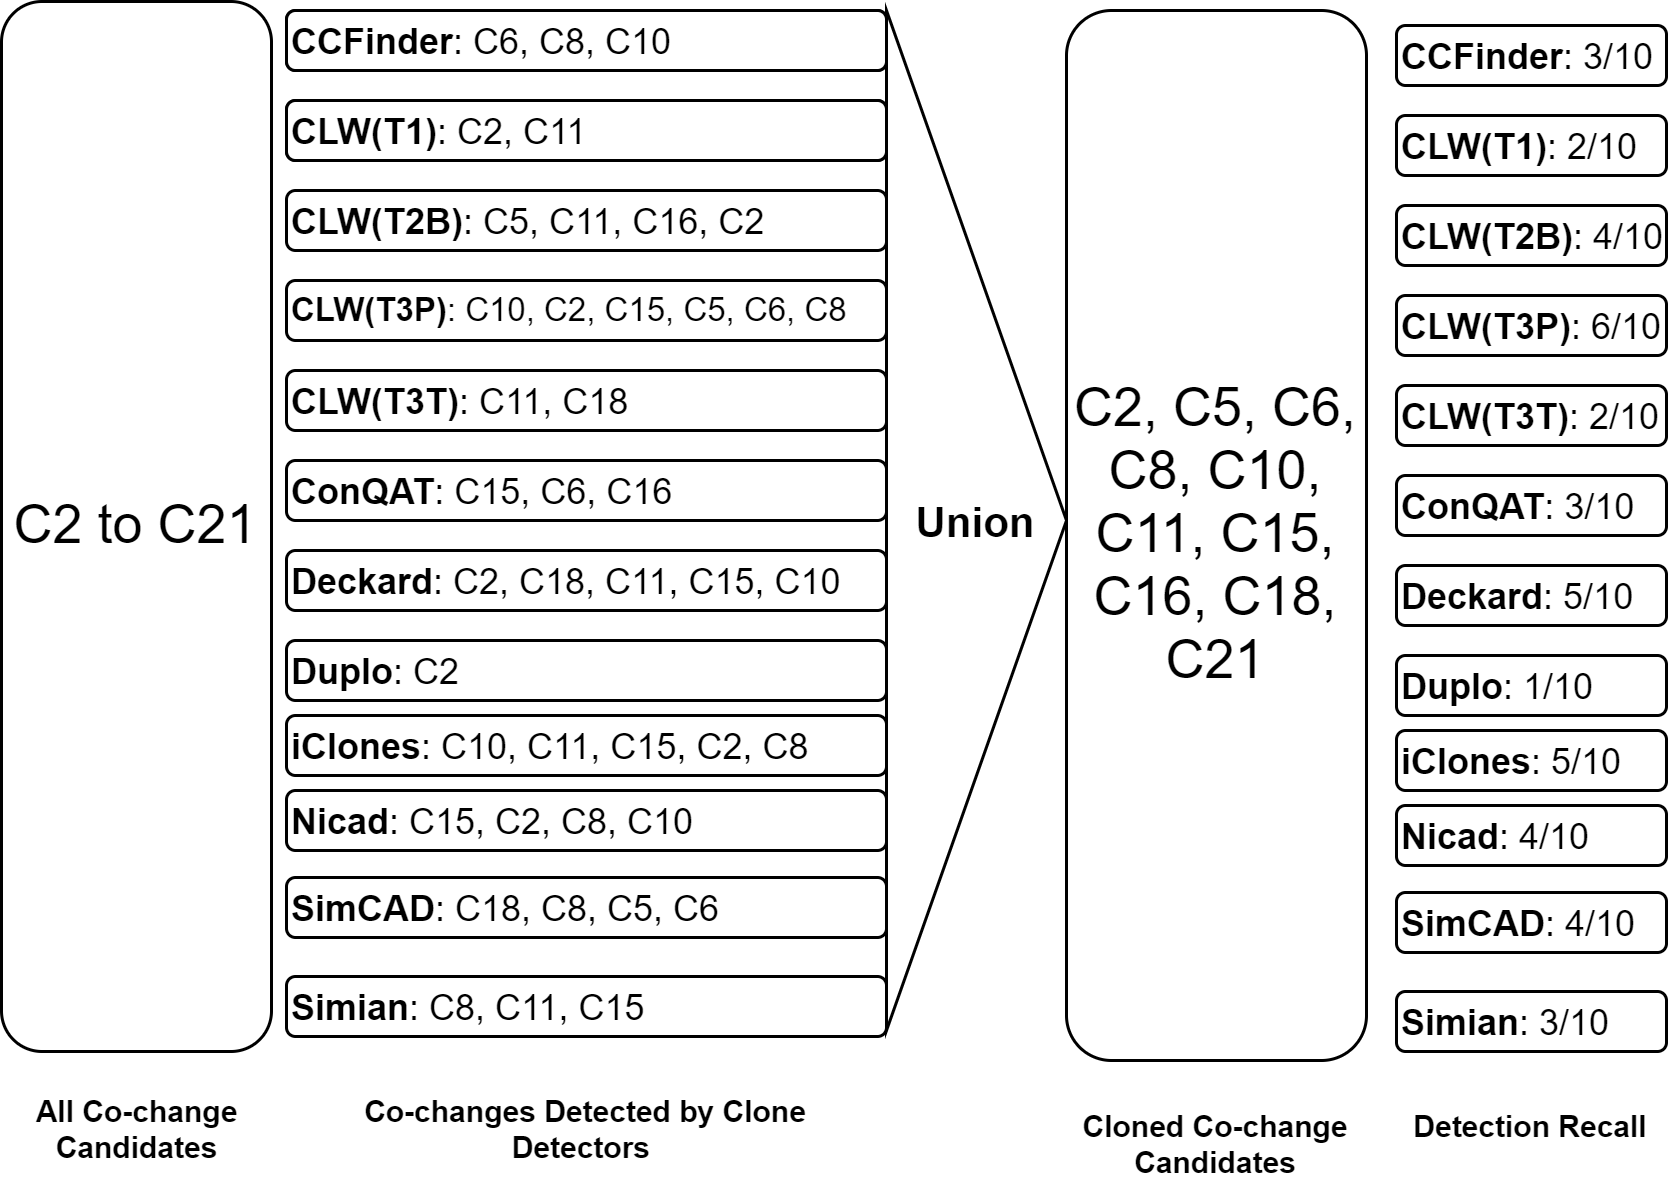
\includegraphics[width=\columnwidth] {CalculatingCC.png}
% Calculation of Change Intersection: SELECT COUNT(`change_id`) FROM `pre_recall_conqat` WHERE `change_detect`>0
\caption{Demonstrating cloned co-change detection process}
\label{fig:CalculatingCC}
\end{figure}
%%% ==================

Based on this study, we tried to answer the following research questions:

\vspace{0.15cm}
\noindent
\textbf{RQ1: }What is the comparison scenario of the clone detectors in predicting cloned co-change candidates?
 
\vspace{0.15cm}
\noindent
\textbf{RQ2: }Why do different clone detectors perform differently in detecting cloned co-change candidates?

\vspace{0.15cm}
\noindent
\textbf{RQ3: }Do the source code processing techniques (Pattern/Token/Text based processing) of the clone detection tools have any impact on their performance in detecting co-change candidates?

\vspace{0.15cm}
\noindent
\textbf{RQ4: }Do clone detection tools designed for detecting different types of clones (Type 1, 2, 3) work differently in detecting cloned co-change candidates?

To the best of our knowledge, our study is the first one to compare clone detection tools considering a particular maintenance perspective (e.g., considering their capabilities in successfully suggesting cloned co-change candidates during software evolution). From an initial assumption, it is obvious that a clone detector which is good in detecting clone should also be good in detecting cloned co-change candidates. In this exploratory study, we wanted to practically verify this assumption. We selected 12 implementations of clone detectors detecting different types of clones in our investigation to verify whether they are also good at detecting co-change candidates. According to our investigation and analysis, we find that, the clone detectors which detects more type-3 clones and performs pattern based source code processing are good in detecting cloned co-change candidates. Our investigation also shows that, tools which provides more number of clone fragments and covers more source code lines are also good in detecting cloned co-change candidates. We have created two rank lists of the clone detection tools based on our investigation. One of them in Table \ref{tab:final-ranking-sum-of-ranks} where we have considered the ranking of the clone detectors in each of the subject systems. A clone detector which performed good in most of the subject system got the higher rank in this ranking table. Other ranking is in Table \ref{tab:final-ranking-wa} where we considered the weighted average (number of changes whose co-change candidates are detected are the weight factor) of F1~Scores of clone detectors considering all the subject systems. Considering both the rankings we find common tools obtaining in top-5 positions. Three of them are the different configurations of CloneWorks except Type-1, and other two clone detectors are Deckard and CCFinder. Therefore, we can conclude that, to detect cloned co-change candidates, those five tools (all are pattern and token based) are the best choice compared to the other seven tools used in this study. From these ranking, we can also find that, text based clone detectors (such as Duplo or CloneWorks Type-1 configuration) are not good for detecting co-change candidates.  

%\vspace{0.5mm}
We organized this paper in the following sections: Some related works are described in Section \ref{the-related-works}, our methodology is in Section \ref{the-methodology}, we described the experimental result in Section \ref{the-experimental-result}, the discussion is in section \ref{the-discussion}, Section \ref{the-threat-validity} explains some possible threats to validity, and we conclude our paper by mentioning future work in Section \ref{the-conclusion-future-works}.

This paper is a significant extension of our previous work \cite{nadim-iwsc-2020} on detecting cloned co-change candidates using different clone detectors. While in our previous study, we have used six open-source software as subject systems to evaluate the performance of six clone detection tools which have been reported good in detection clone fragments from software source code by recent studies. By answering two research questions, we have been evaluated that, even though a tool which is good in detecting clone fragments from software systems may not be good in detecting cloned co-change candidates. We also investigated and reported two possible reasons for such a difference in the performance of clone detection tools while we are using them to predict co-change fragments. We extend our previous work by answering two additional research questions (RQ3, RQ4) to find a more specific reason for the variation of the performance by clone detectors in detecting co-change candidates. We have also increased the generalizability of the previous study by adding two more software systems as subject system totalling the number of subject systems in six. We have added three more clone detectors (totalling nine clone detectors) including four different configurations of one clone detector (CloneWorks) which makes 12 total clone detector executions. We used different configurations of CloneWorks for targeting different types (Type-1, or Type-2 blind, or Type-3 pattern, Type-3 token) of clones to investigate the effect of those types in our study. Therefore, our implementation has been upgraded from 6X6 to 12X8 (Clone detector X Subject Systems) in the current version of the study. In the current extended version of the study, we have shown that the performance of clone detection tools in detecting cloned co-change fragments not only dependent on the number of clone fragments detected and the line covered in the source file by those fragments but also the type of detected clone and underlying source code processing techniques also have some impact.

 %To extend the number of tools than previous study, we added six additional implementations of clone detection techniques by using three additional tools. New tools added are CloneWorks, CCFinder, and Duplo. CloneWorks have been reported as a fast and flexible clone detector for large-scale near-miss clone detection experiments. CloneWorks provides options to modify it’s configuration files which effects on the source code processing mechanism while detecting the clones. This is important to target specific types (1, 2, or 3) of clone by using this clone detection tool. We have applied four types of different configuration files to detect Type-3 pattern, Type-3 Token, Type-2 Blind, and Type-1 clones by using CloneWorks tool. This provided four additional sets of detected clone result. CCFinder is known as a multilinguistic token-based code clone detection system for large scale source code. Inclusion of CCFinder enriched the variation of detected clone fragments in the extended study. To make more comparison of the performance of type-1 clones in detecting co-change candidates we added Duplo in our study. 


\vspace{2mm}
\section{Related Work}
\label{the-related-works}
%Besides the studies of clone detection approaches, 
There are several studies \citep{jeff-evaluating, Roy09comparisonand, 4288192Comparison, ScenarioBasedComparison} that have been focused on ranking different clone detection tools based on their performance and accuracy in detecting different types of clone fragments. \citet{BaileyBurdComparison} did a study for comparing the performance of three clones and two plagiarism detecting tools based on their precision and recall of the ability to detect duplicated codes in a single file or across different files.  \citet{4288192Comparison} evaluated six clone detection tools based on eight large C and Java programs of almost 850 KLOC and made a framework for comparing different clone detection tools with the data validated by one of its authors.  \citet{EvaluateRefactoring} evaluated three representative clone detection techniques from a refactoring perspective where they provided comparative results in terms of portability, kinds of clone reported, scalability, number of false positive, and number of useless clone detection.   \citet{jeff-evaluating} evaluated eleven modern clone detection tools using four benchmark frameworks and noted ConQAT, iClones, NiCad and SimCAD as very good tools for detecting clones of all the three types (Type-1, Type-2, Type-3). \citet{Roy09comparisonand} did a qualitative comparison and evaluation of the latest clone detection approaches and tools, and made a benchmark called BigCloneBench \citep{BigCloneBenchCKRoyJRCordy} which contains eight million manually validated clone pairs in a large inter-project source dataset of more than 25,000 projects and 365 million lines of code. They categorize, relate and assess different clone detection tools based on two different points of view such as classification based on the overlapping set of attributes in the different code fragments and the scenarios how Type-1, Type-2, Type-3, and Type-4 clones created. They also elaborated the procedure of using the result of their study to select the most suitable clone detection tool or technique in the context of a specific set of areas and limitations. \\
There are some studies which not only proposed a clone detection mechanism but also did a comparison of their proposed technique with some existing techniques. \citet{astDetectionComparisonBellon} provided a technique to detect clone using suffix trees in abstract syntax trees and they also made a comparison to other techniques using the Bellon benchmark for clone detectors. \citet{DucasseStringMatchingCloneBallon} and \citet{CloneIntermediateRepresentationBallon} also utilized Bellon’s framework for measuring the performance of their proposed clone detection tools based on string comparison and intermediate source transformation respectively. \citet{CloneIntermediateRepresentationBallon} showed that their tool is capable of detecting Type-3 clones and their technique is better than the source-based clone detectors based on the value of recall through a slight drop in the precision using Bellon’s corpus where clone group is not complete. Compared to the standalone string and token-based clone detectors, their technique showed a little higher precision.\\
All the studies which compared different clone detectors have been focused on the precision, recall, computational complexity, and memory used or detecting a specific type of clone fragments such as Type-1, Type-2, Type-3, or Type-4 during the detection approach of duplicated code in a code-base. Our study to compare clone detectors is completely different from the previous comparisons. We do not want to compare clone detection tools based on the capability to detect clones. Our point of interest is to detect co-change candidates during the software commit operations. \citet{Mondal-2014-PRC-2597073-2597104rankingCoChange} did a study to predict and rank the co-change candidates by analyzing evolutionary coupling from previously done change history using generated clone fragments by NiCad but they did not consider the result of other clone detection tools and also did not show any comparative study among different clone detection tools in doing such prediction and rank of co-change candidates. This work is an extended version of our previous study \cite{nadim-iwsc-2020} using six clone detection tools on six software systems written in C and Java programming languages to compare those tools based on the performance of detecting clone co-change candidates.  We found no other study which have performed similar comparison of clone detectors. To extend our previous research, we have analyzed the performance of nine clone detection tools in 12 different configurations based on their capabilities in finding co-change candidates during software evolution using their generated clone results. According to our knowledge, this is the first such investigation of performance with clone detection tools. 

%\vspace{1mm}
\section{Methodology}
\label{the-methodology}
We have used eight subject systems listed in Table \ref{tab:subject-systems} and 12 clone detection tools (Table \ref{tab:tool-configurations}) for our analysis. Our analysis aims to rank these clone detection tools based on their performance in successfully suggesting actual co-change candidates (ACC) during the software evolution. Before starting our main analysis, we have to resolve some issues and we have taken the following considerations in this regard. 

\vspace{1mm}
\textbf{Selection of subject systems:} To select subject systems for this study, we considered both the popularity of programming language and availability of a considerable amount of revisions. According to the TIOBE Programming Community index \citep{TIOBE2019} (an indicator of the popularity of programming languages), Java is dominating the list of popular programming languages for more than the last ten years and C is the second most popular programming language within this period. Considering this fact, we wanted to select subject systems written in these two programming languages. Our other consideration was the availability of a considerable amount of revisions of each of the systems. Based on both of the considerations, we have chosen the subject systems listed in Table \ref{tab:subject-systems}. Four of our eight subject systems are written in C programming language and other four are in Java.  To increase the generalizability of the study we have added systems having diverse size and application domains.

%%% Beginning of Subject Systems Table
\begin{table}[h] 
\vspace{2mm}
\caption{\label{tab:subject-systems}\textsc{Subject Systems}}
\centering
\begin{tabular}{|c|c|l|c|}
\hline
\textbf{Systems} & \textbf{Language} & \multicolumn{1}{c|}{\textbf{Domains}} & \textbf{Revisions} \\ \hline
Brlcad           & C              & Computer Aided Design                 & 2115               \\ \hline
Camellia         & C              & Batch Job Server                      & 301                \\ \hline
Carol            & Java           & Game                                  & 1700               \\ \hline
Ctags            & C              & Code Def. Generator                   & 774                \\ \hline
Freecol          & Java           & Game                                  & 1950               \\ \hline
Jabref           & Java           & Reference Manager                     & 1545               \\ \hline
jEdit            & Java           & Text Editor                           & 4000               \\ \hline
Qmailadmin (QMA)       & C              & Mail System Manager                   & 317                \\ \hline
\end{tabular}
\end{table}
%%%--- End of Subject Systems Table

%%% Start of Summary Data
\begin{table}[]
\centering
\caption{\label{tab:data-summary}\textsc{Summary of Data Processed}}
\small\addtolength{\tabcolsep}{-4pt}
\begin{tabular}{|l|c|c|c|c|c|c|c|c|}
\hline
\textbf{\begin{tabular}[c]{@{}l@{}}Revisions/\\ Subject Systems\end{tabular}} & \textbf{Brlcad} & \textbf{Camellia} & \textbf{Carol} & \textbf{Ctags} & \textbf{Freecol} & \textbf{Jabref} & \textbf{jEdit} & \textbf{QMA} \\ \hline
Processed                                                                     & 2113            & 301               & 1700           & 774            & 1001             & 1540            & 215            & 317                                                            \\ \hline
Experiencing change                                                           & 660             & 163               & 454            & 447            & 836              & 860             & 145            & 35                                                             \\ \hline
\begin{tabular}[c]{@{}l@{}}Experiencing more \\ than one change\end{tabular}  & 553             & 155               & 430            & 330            & 833              & 755             & 145            & 25                                                             \\ \hline
\end{tabular}
\end{table}
%%%-------------------------------


\vspace{1mm}
\textbf{Selection of clone detectors:} In this research, we wanted to examine those clone detection tools which are good in detecting all types of clones. To select such tools, we considered some related studies. We have taken CloneWorks \cite{CloneWorks-Jeff} as it is considered as a fast and flexible clone detector for large-scale near-miss clone detection experiments. CloneWorks tool provides the ability to change its processing mechanism by changing its configuration files. We applied four different configurations of CloneWorks to detect Type-3 Pattern, Type-3 Token, Type-2 Blind, and Type-1 clones for investigating the impact of the types of clones in detecting co-change candidates. We included Duplo \cite{DuploCloneDetection} as another type-1 clone detector for making the comparison with type-1 clones of CloneWorks in this investigation.  ConQAT \citep{conqat-clone-detecion}, iClones \cite{4812755iclones}, NiCad \citep{5970189Nicad}, and SimCAD \cite{6613857Simcad} have been reported as very good tools for detecting all types of clones in the study of \citet{jeff-evaluating}. Besides these, CCFinder \cite{CCFinderCloneDetection}, Deckard \cite{4222572Deckard}, iClones and NiCad are often considered as common examples of modern clone detectors that support Type-3 clone detection. CCFinder is known as a multi-linguistic token-based code clone detection system for large scale source code. Inclusion of CCFinder enriched the variation of detected clone fragments in the extended study.  To make more comparison of the performance of type-1 clones in detecting co-change candidates we added Duplo in our study. The reason of taking Simian \cite{simianlink} in our analysis was its ability to find duplicated code by line-by-line textual comparison supporting identifier renaming with a fast detection speed on the large repository and extensive use in several clone studies \cite{simian-used-1, Wang-2013-SBC-2491411-2491420, impact-clone-maintenance, Cheung-clones-javascript, cloning-gnome-project}. NiCad, SimCAD, and Simian are textual similarity-based clone detection tools. Deckard works using tree comparison based technique. CCFinder, ConQAT and iClones are token-based clone detection tools.

\vspace{1mm}
\textbf{Determining if the extracted co-changes are related to each other or not:} Even though we have extracted all the changes between two adjacent revisions (i.e., revision n and n+1), it is not possible to fully guarantee that all the changes are actually co-change candidates of each other. There might be some changes which do not depend on any other changes i.e. they may change independently. The inclusion of such dissimilar changes into our calculation can drop the detection accuracy of clone detectors. To minimize such drops, we excluded those co-changes which are not detected by any of the 12 clone detection techniques in our study. As none of the clone detectors considers them as co-change candidates, we considered those changes as dissimilar or independent changes. 

\vspace{1mm}
\textbf{Ensuring if the configuration parameters of all the clone detection tools identical with each other or not:} As we wanted to compare different clone detectors based on their capability of successfully suggesting co-change candidates, it was important to configure them identically during detecting clones from our subject systems. \citet{Wang-2013-SBC-2491411-2491420} introduced confounding configuration choice problem where the configuration of different tools during clone detection may play a vital role and the result may be best or worst depending on the configuration. Our configuration of different tools is shown in Table \ref{tab:tool-configurations}. We have used similar configurations for each of the tools for obtaining a consistent result. We have taken configuration values similar to \citet{jeff-evaluating} which they conducted to compare different clone detectors based on their efficiency in detecting cloned fragments. We provided 70\% similarity threshold for all the clone detection tools (except Deckard) which takes similarity dissimilarity value as parameter. We have used 85\% as the similarity threshold for Deckard 85\% because we found a lot of unwanted clones in the result if we use the similarity threshold 70\%. These results include a lot of duplicated clone fragments and showing a lot of fragments as a clone to itself several times. We also tried some other percentage values such as 75\%, and 80\% but the detected result of Deckard becomes much desirable when we set it to 85\%. \citet{jeff-evaluating} also used 85\% similarity while running Deckard for Mutation Framework. We have also selected identical parameter values such as the minimum number of tokens, minimum number of lines for different clone detection tools. As we wanted to compare different clone detectors based on their capability of successfully suggesting co-change candidates, it was very important to configure them identically during detecting clones from our subject systems.

\textbf{The overall approach:} Our overall processing is performed in some distinct steps.  Initially, we downloaded all the source files of all the revisions of all the subject systems from their respective SVN repositories. We then applied \textbf{diff} operation between each file of a revision with the respective file in the next revision and extracted the change information such as Name of the File which is changed, the Line where the respective change begins, the Line where the change is ended from the output of \textbf{diff}. We did the change extraction for each of the revision (excluding the last one) of all the subject systems. After detecting all the changes, we started the clone detection on all the revisions of all the subject systems using all the clone detection tools. We started our main analysis to find the accuracy of each of the clone detection tools after having the result of all the clone detectors and change information from all the revisions. 

The mechanism of calculating accuracy is demonstrated in our introduction using Fig. \ref{fig:CalculatingCC}. Suppose, we are examining a particular commit operation. The number of fragments that were changed in this commit operation is $n$. Now, let us consider one of these $n$ fragments as the target fragment. Then the other $n-1$ fragments are the actually co-changed candidates for the target fragment. We excluded the non-cloned co-change candidates using the approach described in the introduction. After this exclusion, we get the \textbf{Actually Cloned Co-change} (ACC) for each of the target fragments. 

Let us assume that the target change fragment intersects a particular clone fragment from a particular clone class. The other fragments in that clone class are considered as the \textbf{Predicted Cloned Co-change} (PCC) candidates. We now determine how many of these PCC intersect with the ACC to obtain the number of detected cloned co-change candidates by the clone detector. 

These counts of predicted and actually co-changed candidates are considered as the \textbf{true positives} to calculate Recall, Precision, and F1~Score. We calculate these using the following equations (Eq. 1, 2, and 3).

\begin{equation}
    Recall = \frac{|PCC \cap ACC|}{|ACC|}
\end{equation}

\begin{equation}
    Precision = \frac{|PCC \cap ACC|}{|PCC|}
\end{equation}

\begin{equation}
    F1~Score = \frac{2 \times Precision \times Recall}{Precision + Recall}
\end{equation}

\vspace{1mm}
We repeat the calculating process of Recall and Precision for all the changes in each of the subjects systems with the detected clone fragments generated by all the clone detection tools. We then calculate F1~Score of the clone detectors for each of the subject systems by taking the average values of Recall and Precision which is reported in Table \ref{tab:detection-f1-score}. We reported both the ranking of the tools considering ranks in each of the subject systems in Table \ref{tab:final-ranking-sum-of-ranks} and ranking considering weighted average of F1~Score in all the subject systems in Table \ref{tab:final-ranking-wa}. To calculate the weighted average of F1~Score of the tools we took the total number of changes is the corresponding weighting factor in each subject system whose co-change is detected by any one of the clone detectors in this study.

%%% TAble Summary of Participating Tools
\begin{table}[]
\centering
\caption{\label{tab:tool-configurations}\textsc{Configuration of Participating Clone Detection Tools}}
%\small\addtolength{\tabcolsep}{-1pt}
\begin{tabular}{ll}
\hline
\multicolumn{1}{|l|}{\textbf{Tools}} & \multicolumn{1}{l|}{\textbf{Configuration   for Clone Detection}}                                                                                      \\ \hline
\multicolumn{1}{|l|}{CCFinder}       & \multicolumn{1}{l|}{min. size: 50 tokens, min. token types: 12}                                                                                        \\ \hline
\multicolumn{1}{|l|}{CLW(T1)}        & \multicolumn{1}{l|}{termsplit=token, termproc=Joiner}                                                                                                  \\ \hline
\multicolumn{1}{|l|}{CLW(T2Blind)}   & \multicolumn{1}{l|}{\begin{tabular}[c]{@{}l@{}}cfproc=rename-blind,   cfproc=abstract literal, \\ termsplit=token, termproc=Joiner\end{tabular}}       \\ \hline
\multicolumn{1}{|l|}{CLW(T3Pattern)} & \multicolumn{1}{l|}{\begin{tabular}[c]{@{}l@{}}cfproc=rename-blind, cfproc=abstract literal,\\ termsplit=line\end{tabular}}                            \\ \hline
\multicolumn{1}{|l|}{CLW(T3Token)}   & \multicolumn{1}{l|}{\begin{tabular}[c]{@{}l@{}}termsplit=token,   termproc=FilterOperators, \\ termproc=FilterSeperators\end{tabular}}                 \\ \hline
\multicolumn{1}{|l|}{ConQAT}         & \multicolumn{1}{l|}{block clones, clone   min-length=5, gap ratio=0.3}                                                                                 \\ \hline
\multicolumn{1}{|l|}{Deckard}        & \multicolumn{1}{l|}{\begin{tabular}[c]{@{}l@{}}min. size: 30   tokens, 5 token stride, \\ min. 85\% similarity\end{tabular}}                           \\ \hline
\multicolumn{1}{|l|}{Duplo}          & \multicolumn{1}{l|}{min. size: 10 lines, min. characters/line:1}                                                                                       \\ \hline
\multicolumn{1}{|l|}{iClones}        & \multicolumn{1}{l|}{\begin{tabular}[c]{@{}l@{}}minimum block: 30, minimum   clone: 50, \\ All Transformation\end{tabular}}                             \\ \hline
\multicolumn{1}{|l|}{Nicad}          & \multicolumn{1}{l|}{\begin{tabular}[c]{@{}l@{}}block clones,   blind renaming, max. threshold=0.3,\\ minimum lines=5, maximum lines=2500\end{tabular}} \\ \hline
\multicolumn{1}{|l|}{SimCAD}         & \multicolumn{1}{l|}{block clones,   Source Transformation= generous}                                                                                   \\ \hline
\multicolumn{1}{|l|}{Simian}         & \multicolumn{1}{l|}{min. size: 5   lines, normalize literals/identifiers}                                                                              \\ \hline
\multicolumn{2}{l}{\textit{\textbf{CLW:} CloneWorks, \textbf{T1/2/3:} Type-1/2/3}}                                                                                                                    
\end{tabular}
\end{table}
%%%--- End of Summary Table
\begin{table}[]
\centering
\caption{\label{tab:summary-atc-acc}\textsc{Summary of Actual Target and Co-change Candidates}}
\begin{tabular}{lcccc}
\hline
\multicolumn{1}{|c|}{\textbf{SS}}    & \multicolumn{1}{c|}{\textbf{\# ATC}} & \multicolumn{1}{c|}{\textbf{\# ACC}}  & \multicolumn{1}{c|}{\textbf{\% ATC}} & \multicolumn{1}{c|}{\textbf{\% ACC}} \\ \hline
\multicolumn{1}{|l|}{Brlcad}         & \multicolumn{1}{c|}{2909}            & \multicolumn{1}{c|}{33578}            & \multicolumn{1}{c|}{7.45}            & \multicolumn{1}{c|}{1.89}            \\ \hline
\multicolumn{1}{|l|}{Camellia}       & \multicolumn{1}{c|}{8052}            & \multicolumn{1}{c|}{346140}           & \multicolumn{1}{c|}{20.61}           & \multicolumn{1}{c|}{19.46}           \\ \hline
\multicolumn{1}{|l|}{Carol}          & \multicolumn{1}{c|}{4582}            & \multicolumn{1}{c|}{254311}           & \multicolumn{1}{c|}{11.73}           & \multicolumn{1}{c|}{14.29}           \\ \hline
\multicolumn{1}{|l|}{Ctags}          & \multicolumn{1}{c|}{718}             & \multicolumn{1}{c|}{3648}             & \multicolumn{1}{c|}{1.84}            & \multicolumn{1}{c|}{0.21}            \\ \hline
\multicolumn{1}{|l|}{Freecol}        & \multicolumn{1}{c|}{6865}            & \multicolumn{1}{c|}{265213}           & \multicolumn{1}{c|}{17.57}           & \multicolumn{1}{c|}{14.91}           \\ \hline
\multicolumn{1}{|l|}{Jabref}         & \multicolumn{1}{c|}{8313}            & \multicolumn{1}{c|}{455469}           & \multicolumn{1}{c|}{21.28}           & \multicolumn{1}{c|}{25.60}           \\ \hline
\multicolumn{1}{|l|}{jEdit}          & \multicolumn{1}{c|}{5122}            & \multicolumn{1}{c|}{323277}           & \multicolumn{1}{c|}{13.11}           & \multicolumn{1}{c|}{18.17}           \\ \hline
\multicolumn{1}{|l|}{QMA}            & \multicolumn{1}{c|}{2508}            & \multicolumn{1}{c|}{97396}            & \multicolumn{1}{c|}{6.42}            & \multicolumn{1}{c|}{5.47}            \\ \hline
\multicolumn{1}{|l|}{\textbf{Total}} & \multicolumn{1}{c|}{\textbf{39069}}  & \multicolumn{1}{c|}{\textbf{1779032}} & \multicolumn{1}{c|}{\textbf{100}} & \multicolumn{1}{c|}{\textbf{100}} \\ \hline
\multicolumn{5}{l}{\textit{\textbf{* SS: Subject Systems}}}                                                                                                                                         \\
\multicolumn{5}{l}{\textit{\textbf{* \# ATC: Number of   Actual Taget Changes}}}                                                                                                                    \\
\multicolumn{5}{l}{\textit{\textbf{* \# ACC: Number of   Actual Co-changes}}}                                                                                                                      
\end{tabular}
\end{table}
%%%--- 

\section{Experimental Result}
\label{the-experimental-result}
In this section, we will answer the research questions based on our overall analysis and obtained results by processing each of the eight subject systems using all the 12 clone detection tool executions. 

\subsection{Answer to the \textbf{RQ1}}
\textbf{What is the comparison scenario of the clone detectors in predicting cloned co-change candidates?}\\

The key experimental results are in Figure \ref{fig:AveragePrecisionRecall}, Table \ref{tab:summary-atc-acc}, Table \ref{tab:detection-f1-score}, Table \ref{tab:final-ranking-sum-of-ranks}, and Table \ref{tab:final-ranking-wa} where Fig. \ref{fig:AveragePrecisionRecall} shows the average Recall and average Precision of each of the clone detection tools. Table \ref{tab:summary-atc-acc} shows the summary of target changes and detected co-change candidates for those target changes in each of the subject systems.  We found the highest and lowest percentage of target change and its cloned co-change candidates from Jabref and Ctags respectively. Table \ref{tab:detection-f1-score} shows the F1~Score of each of the clone detectors in each of the subject systems. The F1~Score is calculated using Equation (3). Our experimental results concluded in Table \ref{tab:final-ranking-sum-of-ranks} which shows that CLW(T3Pattern), CLW(T3Token), and Deckard shows top performance (Rank 1 or 2) in most of the subject systems compared to all the other tools. The summary of the results in the Table \ref{tab:final-ranking-sum-of-ranks} shows that among the subject systems, CLW(T3Pattern) is the best in all the subject systems except Camellia and Freecol where Deckard is showing the best performance. CLW(T3Token) shows the second-best performance in most of the subject systems. An overall observation on individual rankings of different clone detection techniques reveals that CLW(3Pattern), Deckard, CLW(3Token), CCFinder show better performance in most of the subject systems compared to the other clone detectors. On the other hand, Duplo, CLW(Type1) shows worst performance in most of the subject systems. Other tools shows average performance considering individual ranking in different subject systems. We also calculated overall ranking considering weighted average of F1~Scores in individual subject systems which is reported in Table \ref{tab:final-ranking-wa}. Though, in individual ranking in Table \ref{tab:final-ranking-sum-of-ranks} CLW(3Pattern) showed best performance compared to Deckard, weighted average of Deckard become higher in Table \ref{tab:final-ranking-wa} as Deckard obtained much better F1~Score in Camellia than CLW(3Pattern). Camellia has a very high number of target changes (\#ATC in Table \ref{tab:summary-atc-acc}) which makes weighted average of F1~Score higher. CLW(3Pattern) obtained second-highest position in the rank list by obtaining very close weighed average F1~Score to Deckard. CLW(Type1) and Duplo obtained the bottom position in the final rank list. 

As our analysis was based on the clone grouping into class or pair provided by the clone detection tools, we found that the efficiency of clone detection tools in suggesting cloned co-change candidates is mostly dependent on its effectiveness in making clone class/ pair. The tool which groups functionally similar clone fragments into a clone class/ pair effectively can perform well in successfully suggesting cloned co-change candidate(s). Different values of the accuracy of different clone detectors indicate the difference in their efficiency in this research domain. 

%%%--- Bar Chart of Recall
%\vspace{2mm}
\begin{figure}
\centering
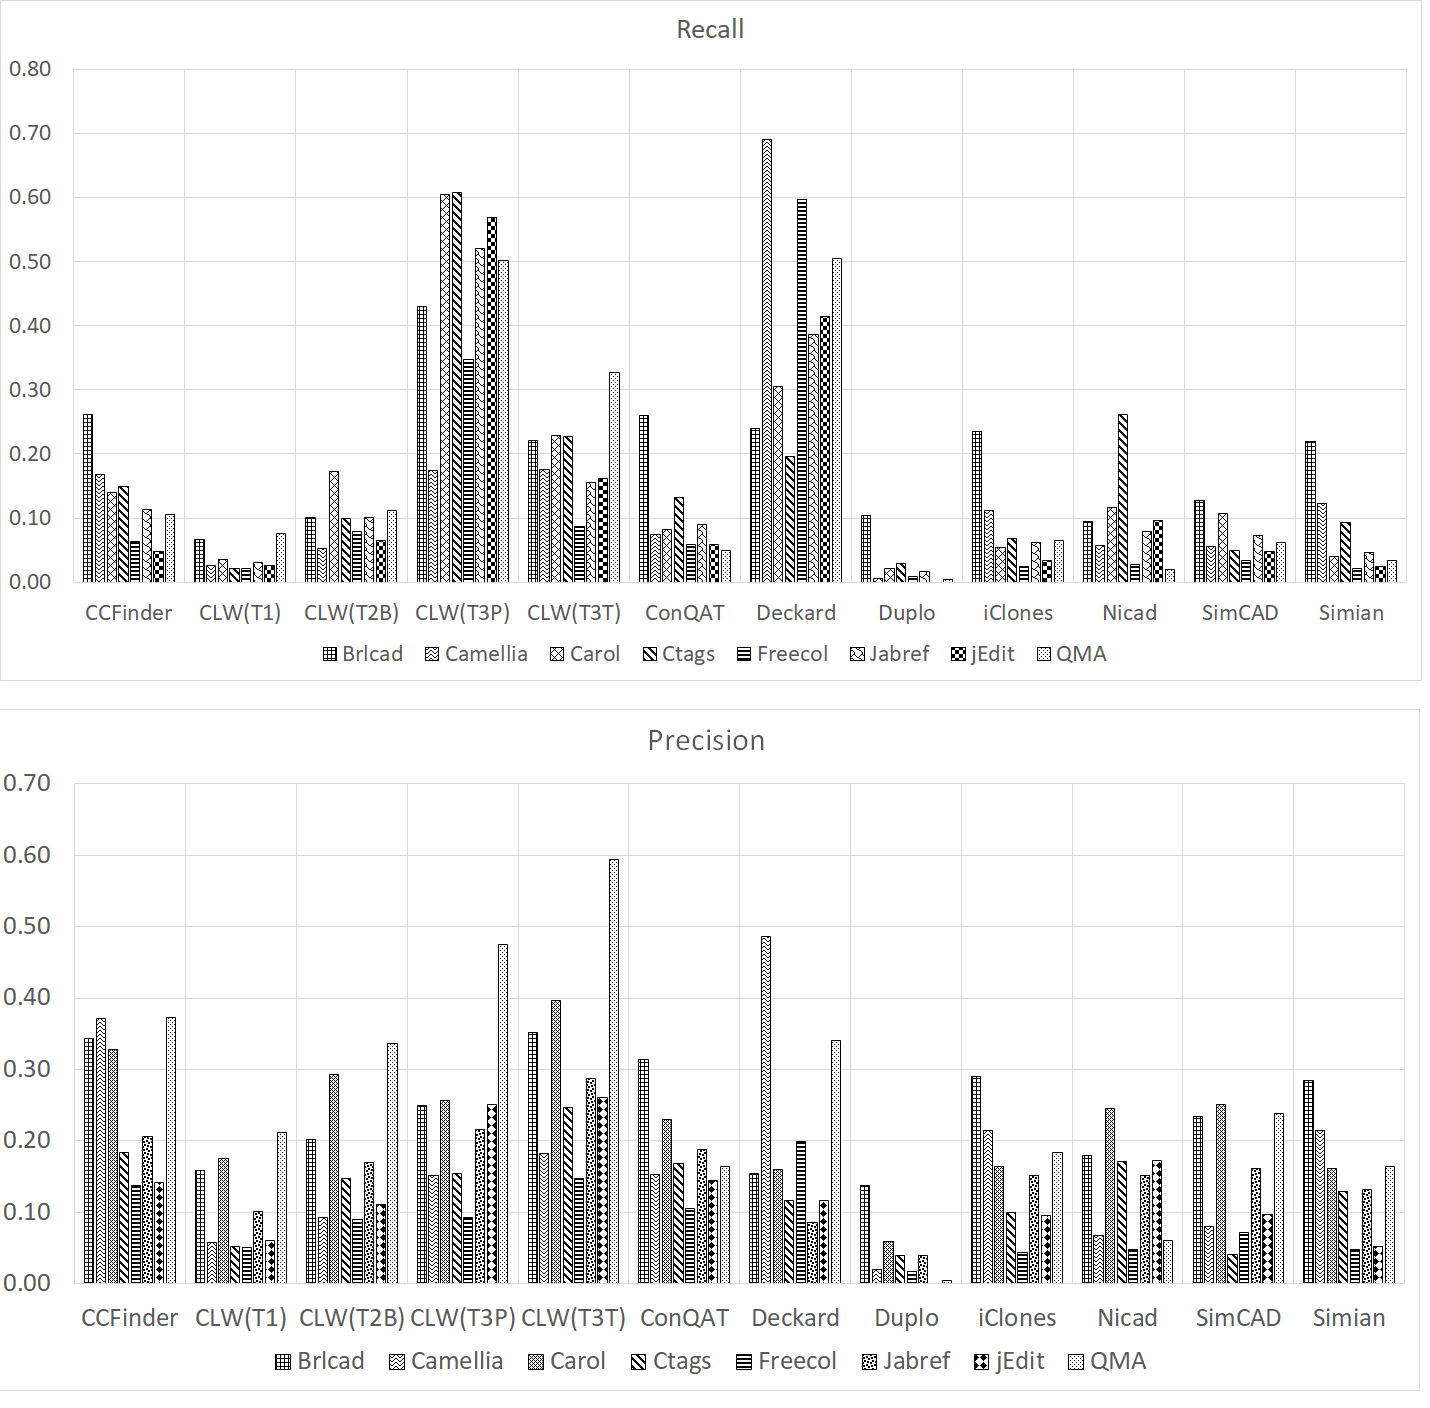
\includegraphics[width=\textwidth] {AveragePrecisionRecall.png}
% Calculation of Change Intersection: SELECT COUNT(`change_id`) FROM `pre_recall_conqat` WHERE `change_detect`>0
\caption{Average precision and recall of different tools}
\label{fig:AveragePrecisionRecall}
\end{figure}
%%% ==================

% %%%--- Bar Chart of Precision
% \vspace{2mm}
% \begin{figure}
% \centering
% 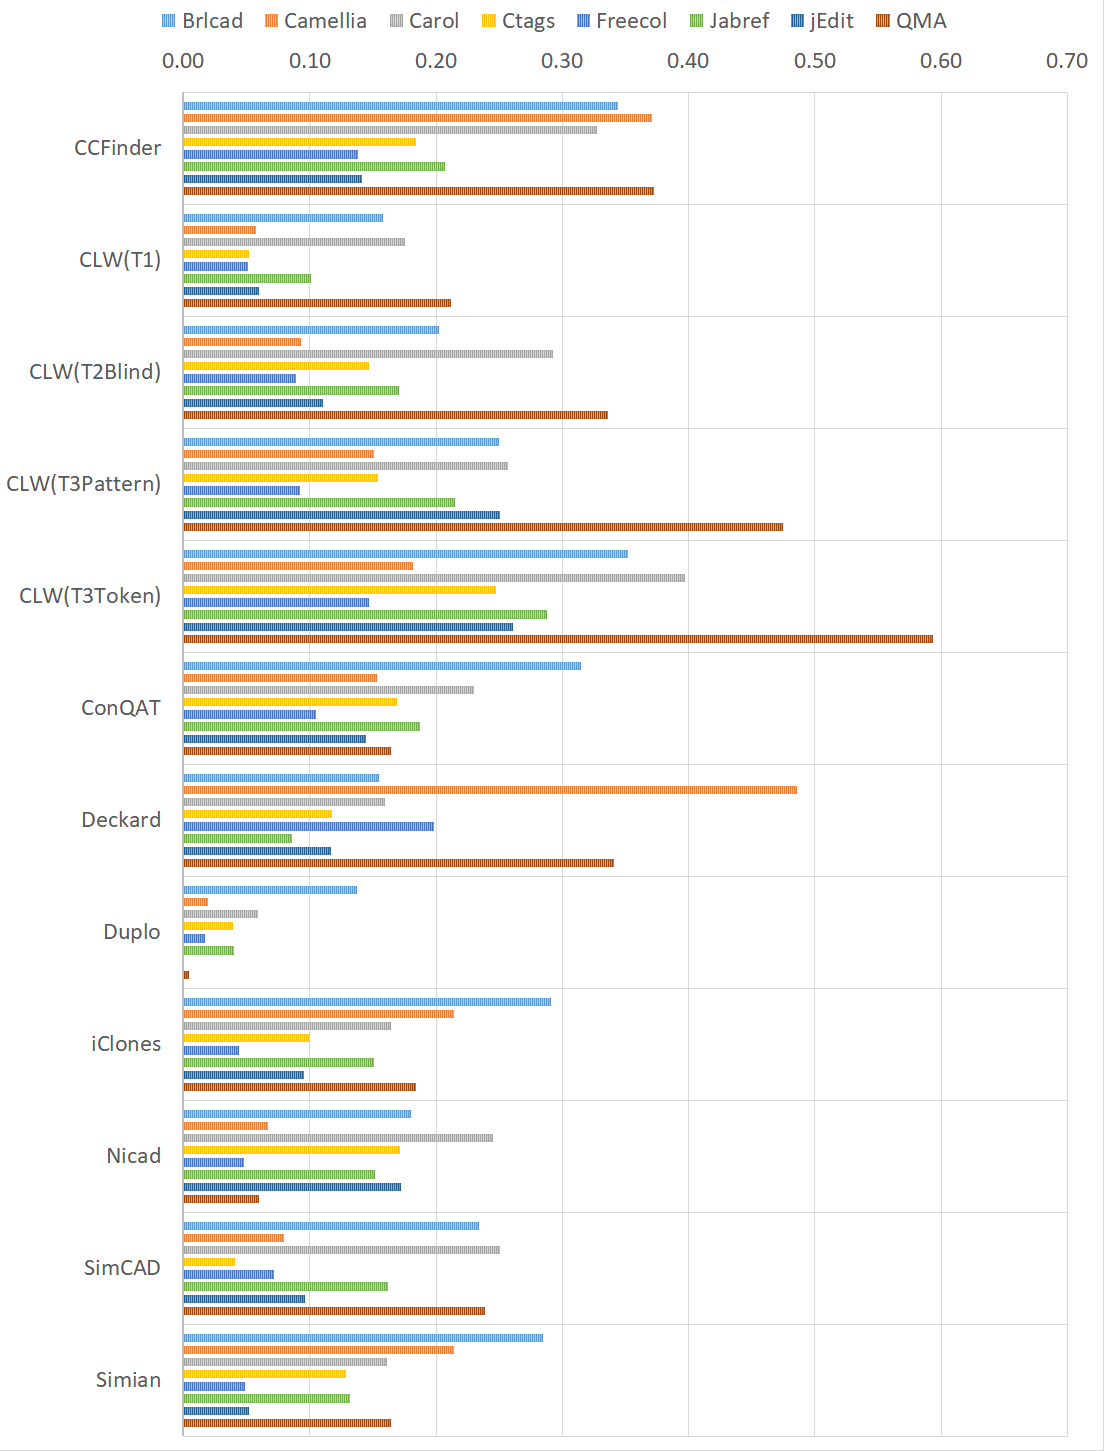
\includegraphics[width=\textwidth] {AveragePrecision.png}
% % Calculation of Change Intersection: SELECT COUNT(`change_id`) FROM `pre_recall_conqat` WHERE `change_detect`>0
% \caption{Average precision of different tools}
% \label{fig:AveragePrecision}
% \end{figure}
% %%% =================

%%%--- Bar Chart of AverageLineCoveredPerSS
\vspace{2mm}
\begin{figure}
\centering
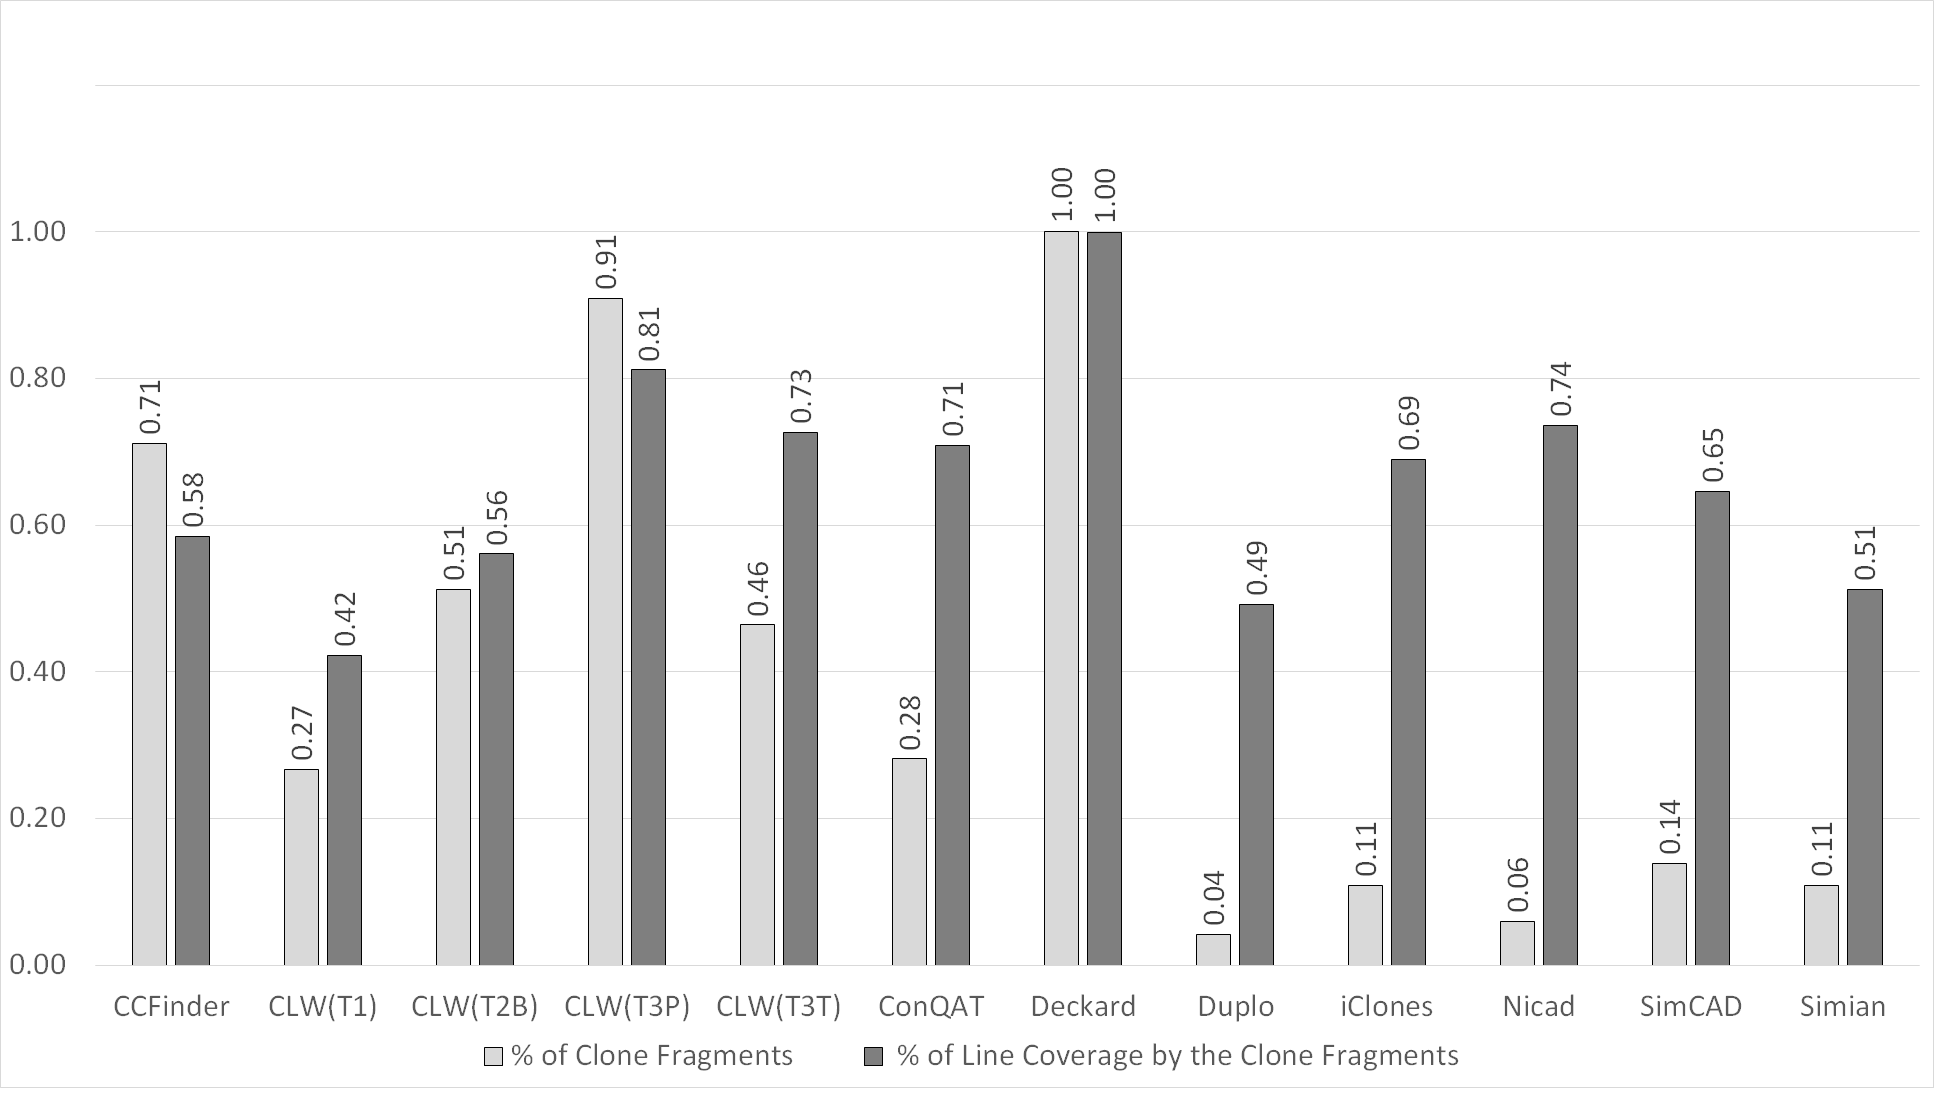
\includegraphics[width=\textwidth] {AverageLineCoveredPerSS.png}
% Calculation of Change Intersection: SELECT COUNT(`change_id`) FROM `pre_recall_conqat` WHERE `change_detect`>0
\caption{Comparing unique line coverage by clone fragments and number of clone fragments from different clone detectors.}
\label{fig:AverageLineCoveredPerSS}
\end{figure}
%%% =================
\subsection{Answer to the \textbf{RQ2}}
\textbf{Why do different clone detectors perform differently in detecting cloned co-change candidates?} \\

From the answer of our \textbf{RQ1}, we found a difference in performance for different clone detection tools in suggesting cloned co-change candidates. We found a clone detection tool which is good in detecting clone fragments may not be good at detecting cloned co-change candidates. This motivates us to find out the reason to answer this research question. 

We investigated the number of clone fragments and the number of unique lines covered by those clone fragments by all the 12 clone detectors from all the revisions of all the subject systems. Figure \ref{fig:AverageLineCoveredPerSS}  shows the comparison scenario of number of clone fragments and line covered by those clone fragments from different clone detectors. For better comparison, we bring the values in a single scale (between 0 and 1) where 0 and 1 represents the lowest and highest values respectively compared to all the clone detectors under comparison. Considering both, the the number of clone fragments and the number of lines covered by those clone fragments from all the revisions of all the subject systems, if we order the clone detectors from the highest to the lowest, we find Deckard and CLW(3Pattern) in the top of the list. CLW(3Token) and CCFinder fall in the respective next position in providing highest number of clone fragments and covering highest number of unique lines in the source files. This scenario shows that, a good clone detector can perform bad in detecting cloned co-change candidates if it does not detect enough clone fragments and does not cover enough unique lines by those clone fragments in the source file. Though, earlier study \cite{Mondal-2014-PRC-2597073-2597104rankingCoChange} suggests that NiCad is a very good clone detector, in both of these cases, it falls at the bottom of the list. Despite, NiCad performs very well in detecting clone fragments, it provides a lower number of clone fragments and also the lower number of line coverage by those clone fragments in the software systems. For that reason, while detecting the cloned co-change candidates, NiCad is showing lower F1~Score. The number of clone fragments and line coverage by those fragments seems to be an underlying factor behind the obtained comparison scenario of the clone detectors in predicting cloned co-change candidates, there can be several other factors such as overlapping of code clones and code similarity detection mechanism. We plan to investigate these factors in future.

\subsection{Answer to the \textbf{RQ3}}
\textbf{Do the source code processing techniques (Pattern/Token/Text based processing) of the clone detection tools have any impact on their performance in detecting co-change candidates?}

We can answer this research question by analysing our final ranking of the clone detectors in Table \ref{tab:final-ranking-sum-of-ranks} and \ref{tab:final-ranking-wa}. Top two clone detectors (Rank 1 and 2) work by extracting source code patterns from the code-base. Deckard first generates vectors from the source file and then extracts tree like source pattern to match similarity among different source code fragments. CLW(3Pattern) also processes the source code terms by splitting in lines and then extracts code patterns. The other five tools (Rank 3 to 7) in the rank list perform token-based source code processing and the remaining five tools perform text based source code processing for detecting clones from the source file. From this result we can say that, text based clone detection tools are not good to be used in detecting cloned co-change candidates during software evolution. The tools which can detect more generalized clone fragments specially pattern based clone detectors are very good for detecting co-change candidates. 

\subsection{Answer to the \textbf{RQ4}}
\textbf{Do clone detection tools designed for detecting different types of clones (Type 1, 2, 3) work differently in detecting cloned co-change candidates?}

From the final rank list of our clone detectors we also find the relation of detected clone types with its ability to detect cloned co-change candidates. Rank list of clone detectors in Table \ref{tab:final-ranking-sum-of-ranks} and \ref{tab:final-ranking-wa} shows that, clone detecting tools such as CLW(Type1), Duplo, which detects only Type 1 clone will not perform good in detecting co-chagne candidates. On the other hand, tools such as Deckard, CLW(3Pattern), CLW(3Token), CCFinder perform very good in detecting cloned co-change candidates. 

%%% Detection F1~Score of Cloned Co-change
\begin{table}[]
\centering
\small\addtolength{\tabcolsep}{-4pt}
\vspace{2mm}
\caption{\textsc{F1~Score of Different Tools in Detecting Cloned Co-change}}
\label{tab:detection-f1-score}
\begin{tabular}{|l|c|c|c|c|c|c|c|c|}
\hline
\multicolumn{1}{|c|}{\textbf{Tools/SS}} & \textbf{Brlcad} & \textbf{Camellia} & \textbf{Carol} & \textbf{Ctags} & \textbf{Freecol} & \textbf{Jabref} & \textbf{jEdit} & \textbf{QMA} \\ \hline
CCFinder                                & 0.30            & 0.23              & 0.20           & 0.16           & 0.09             & 0.15            & 0.07           & 0.16         \\ \hline
CLW(T1)                                 & 0.09            & 0.04              & 0.06           & 0.03           & 0.03             & 0.05            & 0.04           & 0.11         \\ \hline
CLW(T2Blind)                            & 0.13            & 0.07              & 0.22           & 0.12           & 0.08             & 0.13            & 0.08           & 0.17         \\ \hline
CLW(T3Pattern)                          & 0.32            & 0.16              & 0.36           & 0.25           & 0.15             & 0.30            & 0.35           & 0.49         \\ \hline
CLW(T3Token)                            & 0.27            & 0.18              & 0.29           & 0.24           & 0.11             & 0.20            & 0.20           & 0.42         \\ \hline
ConQAT                                  & 0.28            & 0.10              & 0.12           & 0.15           & 0.08             & 0.12            & 0.08           & 0.08         \\ \hline
Deckard                                 & 0.19            & 0.57              & 0.21           & 0.15           & 0.30             & 0.14            & 0.18           & 0.41         \\ \hline
Duplo                                   & 0.12            & 0.01              & 0.03           & 0.03           & 0.01             & 0.02            & 0.00           & 0.00         \\ \hline
iClones                                 & 0.26            & 0.15              & 0.08           & 0.08           & 0.03             & 0.09            & 0.05           & 0.10         \\ \hline
Nicad                                   & 0.12            & 0.06              & 0.16           & 0.21           & 0.04             & 0.10            & 0.12           & 0.03         \\ \hline
SimCAD                                  & 0.17            & 0.07              & 0.15           & 0.04           & 0.05             & 0.10            & 0.06           & 0.10         \\ \hline
Simian                                  & 0.25            & 0.16              & 0.06           & 0.11           & 0.03             & 0.07            & 0.03           & 0.06         \\ \hline
\end{tabular}
\end{table}
%===============================

%%% Ranking Table
\begin{table}[]
\caption{\textsc{Ranks of the clone detectors by considering individual ranking in each of the Subject Systems}}
\label{tab:final-ranking-sum-of-ranks}
\centering
\addtolength{\tabcolsep}{0pt}
\begin{tabular}{lcccccccccc}
\hline
\multicolumn{1}{|c|}{\textbf{\begin{tabular}[c]{@{}c@{}}Tools/\\ Subject Systems\end{tabular}}} & \multicolumn{1}{c|}{\textbf{S1}} & \multicolumn{1}{c|}{\textbf{S2}} & \multicolumn{1}{c|}{\textbf{S3}} & \multicolumn{1}{c|}{\textbf{S4}} & \multicolumn{1}{c|}{\textbf{S5}} & \multicolumn{1}{c|}{\textbf{S6}} & \multicolumn{1}{c|}{\textbf{S7}} & \multicolumn{1}{c|}{\textbf{S8}} & \multicolumn{1}{c|}{\textbf{\begin{tabular}[c]{@{}c@{}}Sum of \\ Ranks\end{tabular}}} & \multicolumn{1}{c|}{\textbf{\begin{tabular}[c]{@{}c@{}}Final\\ Rank\end{tabular}}} \\ \hline
\multicolumn{1}{|l|}{\textbf{CLW(T3Pattern)}}                                                   & \multicolumn{1}{c|}{1}           & \multicolumn{1}{c|}{4}           & \multicolumn{1}{c|}{1}           & \multicolumn{1}{c|}{1}           & \multicolumn{1}{c|}{2}           & \multicolumn{1}{c|}{1}           & \multicolumn{1}{c|}{1}           & \multicolumn{1}{c|}{1}           & \multicolumn{1}{c|}{12}                                                               & \multicolumn{1}{c|}{\textbf{1}}                                                    \\ \hline
\multicolumn{1}{|l|}{\textbf{CLW(T3Token)}}                                                     & \multicolumn{1}{c|}{4}           & \multicolumn{1}{c|}{3}           & \multicolumn{1}{c|}{2}           & \multicolumn{1}{c|}{2}           & \multicolumn{1}{c|}{3}           & \multicolumn{1}{c|}{2}           & \multicolumn{1}{c|}{2}           & \multicolumn{1}{c|}{2}           & \multicolumn{1}{c|}{20}                                                               & \multicolumn{1}{c|}{\textbf{2}}                                                    \\ \hline
\multicolumn{1}{|l|}{\textbf{Deckard}}                                                          & \multicolumn{1}{c|}{7}           & \multicolumn{1}{c|}{1}           & \multicolumn{1}{c|}{4}           & \multicolumn{1}{c|}{6}           & \multicolumn{1}{c|}{1}           & \multicolumn{1}{c|}{4}           & \multicolumn{1}{c|}{3}           & \multicolumn{1}{c|}{3}           & \multicolumn{1}{c|}{29}                                                               & \multicolumn{1}{c|}{\textbf{3}}                                                    \\ \hline
\multicolumn{1}{|l|}{\textbf{CCFinder}}                                                         & \multicolumn{1}{c|}{2}           & \multicolumn{1}{c|}{2}           & \multicolumn{1}{c|}{5}           & \multicolumn{1}{c|}{4}           & \multicolumn{1}{c|}{4}           & \multicolumn{1}{c|}{3}           & \multicolumn{1}{c|}{7}           & \multicolumn{1}{c|}{5}           & \multicolumn{1}{c|}{32}                                                               & \multicolumn{1}{c|}{\textbf{4}}                                                    \\ \hline
\multicolumn{1}{|l|}{\textbf{CLW(T2Blind)}}                                                     & \multicolumn{1}{c|}{9}           & \multicolumn{1}{c|}{8}           & \multicolumn{1}{c|}{3}           & \multicolumn{1}{c|}{7}           & \multicolumn{1}{c|}{5}           & \multicolumn{1}{c|}{5}           & \multicolumn{1}{c|}{5}           & \multicolumn{1}{c|}{4}           & \multicolumn{1}{c|}{46}                                                               & \multicolumn{1}{c|}{\textbf{5}}                                                    \\ \hline
\multicolumn{1}{|l|}{\textbf{ConQAT}}                                                           & \multicolumn{1}{c|}{3}           & \multicolumn{1}{c|}{7}           & \multicolumn{1}{c|}{8}           & \multicolumn{1}{c|}{5}           & \multicolumn{1}{c|}{6}           & \multicolumn{1}{c|}{6}           & \multicolumn{1}{c|}{6}           & \multicolumn{1}{c|}{9}           & \multicolumn{1}{c|}{50}                                                               & \multicolumn{1}{c|}{\textbf{6}}                                                    \\ \hline
\multicolumn{1}{|l|}{\textbf{iClones}}                                                          & \multicolumn{1}{c|}{11}          & \multicolumn{1}{c|}{10}          & \multicolumn{1}{c|}{6}           & \multicolumn{1}{c|}{3}           & \multicolumn{1}{c|}{8}           & \multicolumn{1}{c|}{7}           & \multicolumn{1}{c|}{4}           & \multicolumn{1}{c|}{11}          & \multicolumn{1}{c|}{60}                                                               & \multicolumn{1}{c|}{\textbf{7}}                                                    \\ \hline
\multicolumn{1}{|l|}{\textbf{Simian}}                                                           & \multicolumn{1}{c|}{5}           & \multicolumn{1}{c|}{6}           & \multicolumn{1}{c|}{9}           & \multicolumn{1}{c|}{9}           & \multicolumn{1}{c|}{10}          & \multicolumn{1}{c|}{9}           & \multicolumn{1}{c|}{9}           & \multicolumn{1}{c|}{7}           & \multicolumn{1}{c|}{64}                                                               & \multicolumn{1}{c|}{\textbf{8}}                                                    \\ \hline
\multicolumn{1}{|l|}{\textbf{Nicad}}                                                            & \multicolumn{1}{c|}{8}           & \multicolumn{1}{c|}{9}           & \multicolumn{1}{c|}{7}           & \multicolumn{1}{c|}{10}          & \multicolumn{1}{c|}{7}           & \multicolumn{1}{c|}{8}           & \multicolumn{1}{c|}{8}           & \multicolumn{1}{c|}{8}           & \multicolumn{1}{c|}{65}                                                               & \multicolumn{1}{c|}{\textbf{9}}                                                    \\ \hline
\multicolumn{1}{|l|}{\textbf{SimCAD}}                                                           & \multicolumn{1}{c|}{6}           & \multicolumn{1}{c|}{5}           & \multicolumn{1}{c|}{11}          & \multicolumn{1}{c|}{8}           & \multicolumn{1}{c|}{11}          & \multicolumn{1}{c|}{10}          & \multicolumn{1}{c|}{11}          & \multicolumn{1}{c|}{10}          & \multicolumn{1}{c|}{72}                                                               & \multicolumn{1}{c|}{\textbf{10}}                                                   \\ \hline
\multicolumn{1}{|l|}{\textbf{CLW(T1)}}                                                          & \multicolumn{1}{c|}{12}          & \multicolumn{1}{c|}{11}          & \multicolumn{1}{c|}{10}          & \multicolumn{1}{c|}{11}          & \multicolumn{1}{c|}{9}           & \multicolumn{1}{c|}{11}          & \multicolumn{1}{c|}{10}          & \multicolumn{1}{c|}{6}           & \multicolumn{1}{c|}{80}                                                               & \multicolumn{1}{c|}{\textbf{11}}                                                   \\ \hline
\multicolumn{1}{|l|}{\textbf{Duplo}}                                                            & \multicolumn{1}{c|}{10}          & \multicolumn{1}{c|}{12}          & \multicolumn{1}{c|}{12}          & \multicolumn{1}{c|}{12}          & \multicolumn{1}{c|}{12}          & \multicolumn{1}{c|}{12}          & \multicolumn{1}{c|}{12}          & \multicolumn{1}{c|}{12}          & \multicolumn{1}{c|}{94}                                                               & \multicolumn{1}{c|}{\textbf{12}}                                                   \\ \hline
\multicolumn{11}{l}{\textit{\textbf{\begin{tabular}[c]{@{}l@{}}* S1-S8 represents sequence of eight subject systems used in this study.\end{tabular}}}}                                                                                                                                                                                                                                                                                                                                                                                                          
\end{tabular}
\end{table}
%%% ==================================================

%%% --- Final Ranking ---------------------
\begin{table}[]
\caption{\label{tab:final-ranking-wa}\textsc{Ranks of the clone detectors by considering weighted average F1~Score in all the subject systems}}
\centering
\begin{tabular}{|c|c|c|c|c|}
\hline
\textbf{\begin{tabular}[c]{@{}c@{}}Clone \\ Detectors\end{tabular}} & \textbf{\begin{tabular}[c]{@{}c@{}}WA of\\ Precision (p)\end{tabular}} & \textbf{\begin{tabular}[c]{@{}c@{}}WA of \\ Recall (r)\end{tabular}} & \textbf{\begin{tabular}[c]{@{}c@{}}F1 Score\\ 2pr/(p+r)\end{tabular}} & \multicolumn{1}{l|}{\textbf{\begin{tabular}[c]{@{}l@{}}Final\\ Rank\end{tabular}}} \\ \hline
Deckard                                                             & 0.22                                                                   & 0.47                                                                 & \textbf{0.30}                                                         & \textbf{1}                                                                         \\ \hline
CLW(3Pattern)                                                       & 0.21                                                                   & 0.43                                                                 & \textbf{0.28}                                                         & \textbf{2}                                                                         \\ \hline
CLW(3Token)                                                         & 0.27                                                                   & 0.17                                                                 & \textbf{0.21}                                                         & \textbf{3}                                                                         \\ \hline
CCFinder                                                            & 0.25                                                                   & 0.12                                                                 & \textbf{0.16}                                                         & \textbf{4}                                                                         \\ \hline
CLW(2Blind)                                                         & 0.16                                                                   & 0.09                                                                 & \textbf{0.12}                                                         & \textbf{5}                                                                         \\ \hline
ConQAT                                                              & 0.17                                                                   & 0.09                                                                 & \textbf{0.12}                                                         & \textbf{6}                                                                         \\ \hline
iClones                                                             & 0.15                                                                   & 0.07                                                                 & \textbf{0.10}                                                         & \textbf{7}                                                                         \\ \hline
Nicad                                                               & 0.13                                                                   & 0.07                                                                 & \textbf{0.09}                                                         & \textbf{8}                                                                         \\ \hline
Simian                                                              & 0.14                                                                   & 0.07                                                                 & \textbf{0.09}                                                         & \textbf{9}                                                                         \\ \hline
SimCAD                                                              & 0.14                                                                   & 0.07                                                                 & \textbf{0.09}                                                         & \textbf{10}                                                                        \\ \hline
CLW(Type1)                                                          & 0.10                                                                   & 0.03                                                                 & \textbf{0.05}                                                         & \textbf{11}                                                                        \\ \hline
Duplo                                                               & 0.03                                                                   & 0.02                                                                 & \textbf{0.02}                                                         & \textbf{12}                                                                        \\ \hline
\end{tabular}
\end{table}
% ======================================================================

\vspace{2mm}
\section{Discussion}
\label{the-discussion}
There are two primary perspectives of managing code clones: (1) clone tracking and (2) clone refactoring. Our research essentially focuses on the clone tracking perspective. The main task of a clone tracker is to suggest similar co-change candidates when a programmer attempts to change a code fragment. For suggesting co-change candidates, a clone tracker depends on a clone detector. Our research compares 12 promising clone detectors based on their capabilities in suggesting cloned co-change candidates. According to our investigation, CloneWorks (Type-2 and 3), Deckard, and CCFinder are the most promising tools for suggesting such co-change candidates based on the both rankings we obtained in Table \ref{tab:final-ranking-sum-of-ranks} and Table \ref{tab:final-ranking-wa}. Based on our overall observation, we can say that the performance of CloneWorks (Type-3 Pattern/ Token) and Deckard are much better compared to the other clone detection tools in detecting co-change candidates during software evolution. As the clone classes/ pairs generated by different clone detectors played an important role in our analysis, we can say that the clone detectors which can group similar clone fragments into a class efficiently will perform better in detecting co-change candidates during the commit operation. From our findings we can also say that the clone detectors which detect all the Type 1, 2, 3 clones are also perform good in detecting co-cahange candidates. 

%Therefore, from these observation, we can conclude that the performance of Deckard, ConQAT, and NiCad is better compared to the other clone detectors in grouping similar clone fragments into a clone class.

\vspace{1mm}
When a particular code fragment is changed, we apply the clone detectors to predict which other similar code fragments might also need to be co-changed. However, some dissimilar fragments might also be changed together with the particular fragment. As we are applying only clone detectors, we cannot consider those dissimilar co-change candidates in our research.

\vspace{1mm}
In our research, we do not compare the clone detectors considering their clone detection efficiency. We rather compare the clone detection tools based on their ability in suggesting cloned co-change candidates. Such a comparison of clone detectors focusing on a particular maintenance perspective was not done previously. Suggesting co-change candidates for a target program entity is an important impact analysis \citep{book-change-impact} task during software evolution. Thus, through our research, we investigate which of the clone detectors can be useful in change impact analysis to what extent. Findings from our research can identify which clone detector(s) can be promising for change impact analysis. 

\vspace{2mm}
\section{Threats to Validity}
\label{the-threat-validity}
We have investigated eight subject systems in our study. While more subject systems could generalize our findings, we selected our systems focusing on their diversity, popularity of used programming language, and availability of a considerable number of revisions. For example, our systems are of different application domains, sizes, and revision history lengths. Thus, our findings are not biased by our choice of subject systems. We believe that our findings are important from the perspectives of software maintenance.

We have investigated 12 different configuration of nine clone detectors in our study. 
Detection parameter settings of the clone detectors can have an impact on their comparison. However, the parameters of different clone detectors were selected considering their equivalence. Thus, we believe that we have a fair comparison among the clone detectors.

Several code fragments might change together in a commit operation. While some of these fragments can be similar to one another, and some might be dissimilar. Similar code fragments co-change (i.e., change together) for ensuring consistency of the code-base. However, dissimilar code fragments can co-change because of their underlying dependencies which could have some impact on the generalization of this research outcome. As we aim to compare the clone detection tools, we wanted to discard the dissimilar co-change candidates from our consideration. If a co-change candidate was not detected as a true positive by any of the clone detectors, we discarded the candidate. We believe that such a consideration is reasonable in our experiment aiming towards comparing clone detectors and our findings may inspire more similar research.

\vspace{2mm}
\section{Conclusion and Future Works}
\label{the-conclusion-future-works}
In this research, we make a comparison among different clone detection tools from the perspective of software maintenance. In particular, we investigate their performances in successfully suggesting (i.e., predicting) cloned co-change candidates during evolution. We used eight open source subject systems written in C and Java for our analysis. According to our findings (Table \ref{tab:final-ranking-sum-of-ranks} \& \ref{tab:final-ranking-wa}) on thousands of revisions of these systems, CloneWorks (Type-3) and Deckard show the most promising results in most of the eight subject systems compared to the other tools. CCFinder and CloneWorks (Type-2) are also shows better performance in some of the subject systems. Although we have figured some reasons of the better performance of Deckard, CloneWorks, and CCFinder in the Discussion section of our study, we planned to extend this research by analyzing the clone detection mechanism of the clone detectors to find out some other reasons for their performance. We also want to investigate the impact of different similarity score of different clone detectors in finding co-change candidates in our future studies. Besides this, we want to include some other clone detection tools of different detection mechanism (i.e., tree/ token/ text-based) and subject systems written in some different programming languages (i.e. C/ C++, C\#, Python) for extending our research. %\\ \\

\section*{Acknowledgment}
This research is supported by the Natural Sciences and Engineering Research Council of Canada (NSERC), and by a Canada First Research Excellence Fund (CFREF) grant coordinated by the Global Institute for Food Security (GIFS).

%\section*{References}
\bibliography{mybibfile}

\end{document}